\begin{figure}
    \centering
    \begin{subfigure}[b]{0.8\linewidth}
        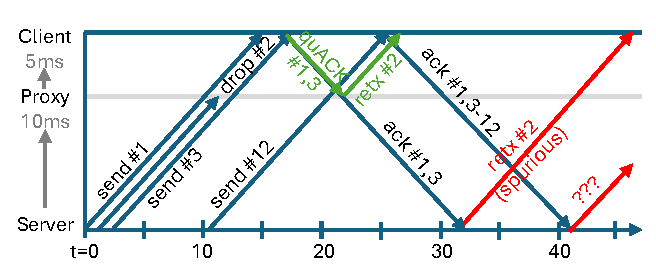
\includegraphics[width=\linewidth, trim=0 10 0 10, clip]{packrat/figures/reordering_unmodified.pdf}
        \caption{Unmodified ACK.}
        \label{fig:packrat:reordering:unmodified}
    \end{subfigure}
    \begin{subfigure}[b]{0.8\linewidth}
        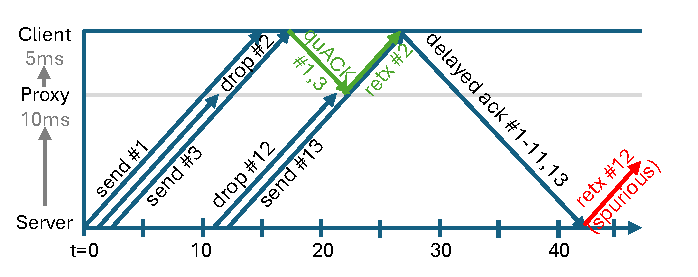
\includegraphics[width=\linewidth, trim=0 9 0 10, clip]{packrat/figures/reordering_delayed_ack.pdf}
        \caption{Na\"ive delayed ACK.}
        \label{fig:packrat:reordering:delayed-ack}
    \end{subfigure}
    \begin{subfigure}[b]{0.8\linewidth}
        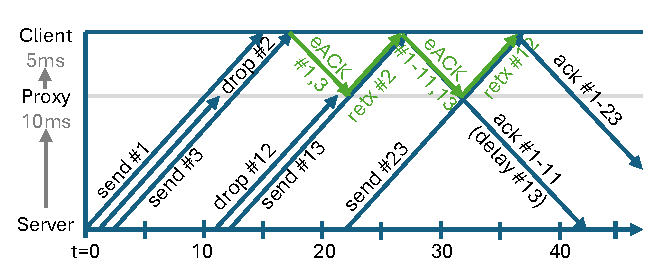
\includegraphics[width=\linewidth, trim=0 9 0 10, clip]{packrat/figures/reordering_with_signal.pdf}
        \caption{ACK with Packrat reorder delay of 10 ms.}
        \label{fig:packrat:reordering:packrat}
    \end{subfigure}
    \caption{The reordering problem where in-network retransmissions with
    millisecond RTTs cause the server to send spurious retransmissions. The
    end-to-end ACKs constructed with a Packrat reorder delay prevent this problem.
    }
    \label{fig:packrat:reordering}
\end{figure}
